\section{Negation in \textsl{Prolog}}
In diesem Abschnitt besprechen wir die Implementierung des Negations-Operators in
\textsl{Prolog}.  Wir zeigen zunächst anhand eines einfachen Beispiels die Verwendung
dieses Operators, besprechen dann seine Semantik und zeigen abschließend, in welchen
Fällen die Verwendung des Negations-Operators problematisch ist.

\subsection{Berechnung der Differenz zweier Listen}
In \textsl{Prolog} wird der Negations-Operator als ``\texttt{\symbol{92}+}'' geschrieben.
Wir erläutern die Verwendung dieses 
Operators am Beispiel einer Funktion, die die Differenz zweier Mengen berechnen soll,
wobei die Mengen durch Listen dargestellt werden.  Wir werden  die Funktion \\[0.1cm]
\hspace*{1.3cm} 
$\texttt{difference}: \textsl{List}(\textsl{Number}) \times \textsl{List}(\textsl{Number}) \rightarrow \textsl{List}(\textsl{Number})$
\\[0.1cm]
durch bedingte Gleichungen spezifizieren.  Der Ausdruck \\[0.1cm]
\hspace*{1.3cm} $\mathtt{difference}(l_1,l_2)$ \\[0.1cm]
berechnet die Liste aller der Elemente aus $l_1$, die nicht Elemente der Liste $l_2$ sind.
In \textsc{SetlX} könnten wir diese Funktion wie in Abbildung \ref{fig:difference.stl}
gezeigt implementieren.
\begin{figure}[!ht]
\centering
\begin{Verbatim}[ frame         = lines, 
                  framesep      = 0.3cm, 
                  labelposition = bottomline,
                  numbers       = left,
                  numbersep     = -0.2cm,
                  xleftmargin   = 0.8cm,
                  xrightmargin  = 0.8cm,
                ]
    difference := procedure(l1, l2) {
        return [ x in l1 | !(x in l2) ];
    };
\end{Verbatim}
\vspace*{-0.3cm}
\caption{Implementierung der Prozedur \texttt{difference} in \textsc{SetlX}.}
\label{fig:difference.stl}
\end{figure}

\noindent
In \textsl{Prolog} erfolgt die Implementierung dieser Funktion durch Rekursion im ersten Argument.
Dazu stellen wir zunächst bedingte Gleichungen auf:
\begin{enumerate}
\item $\textsl{difference}([], l) = []$.
\item $\neg \textsl{member}(h, l) \rightarrow \textsl{difference}([h|t], l) = [h |\textsl{difference}(t,l)]$,

      denn wenn das Element $h$ in der Liste $l$ nicht vorkommt, so bleibt dieses Element
      im Ergebnis erhalten.
\item $     \textsl{member}(h, l) \rightarrow \textsl{difference}([h|t], l) = \textsl{difference}(t,l)$.
\end{enumerate}

\begin{figure}[!h]
  \centering
\begin{Verbatim}[ frame         = lines, 
                  framesep      = 0.3cm, 
                  labelposition = bottomline,
                  numbers       = left,
                  numbersep     = -0.2cm,
                  xleftmargin   = 0.8cm,
                  xrightmargin  = 0.8cm
                ]
    % difference( +List(Number), +List(Number), -List(Number) ).
    difference( [], _L, [] ).
    
    difference( [ H | T ], L, [ H | R ] ) :-
    	\+ member( H, L ),
    	difference( T, L, R ).
    
    difference( [ H | T ], L, R ) :-
    	member( H, L ),
    	difference( T, L, R ).
\end{Verbatim}
\vspace*{-0.3cm}
  \caption{Berechnung der Differenz zweier Listen}
  \label{fig:difference}
\end{figure}

\subsection{Semantik des Negations-Operators in \textsc{Prolog}}
Es bleibt zu klären, wie das \textsl{Prolog}-System eine Anfrage der Form
\\[0.1cm]
\hspace*{1.3cm} \texttt{\symbol{92}+} $A$ \\[0.1cm]
beantwortet, wie also der \texttt{not}-Operator implementiert ist.
\begin{enumerate}
\item Zunächst versucht das System, die Anfrage ``$A$'' zu beantworten.
\item Falls die Beantwortung der Anfrage ``$A$'' scheitert, ist die Beantwortung
      der Anfrage ``\texttt{\symbol{92}+} $A$'' erfolgreich.  In diesem Fall werden keine
      Variablen instanziiert.
\item Falls die Beantwortung der Anfrage ``$A$'' erfolgreich ist, so scheitert die Beantwortung
      der Anfrage ``\texttt{\symbol{92}+} $A$''.
\end{enumerate}

Wichtig ist zu sehen, dass bei der Beantwortung einer negierten Anfrage in keinem Fall
Variablen instanziiert werden.  Eine negierte Anfrage
\\[0.1cm]
\hspace*{1.3cm} \texttt{\symbol{92}+} $A$ \\[0.1cm]
funktioniert daher nur dann wie erwartet, wenn die Anfrage $A$ keine Variablen mehr
enthält.  Zur Illustration betrachten wir das Programm in Abbildung \ref{fig:not-problem}.
Versuchen wir mit diesem Programm die Anfrage \\[0.1cm]
\hspace*{1.3cm} \texttt{smart1(X)} \\[0.1cm]
zu beantworten, so wird diese Anfrage reduziert zu der Anfrage \\[0.1cm]
\hspace*{1.3cm} \texttt{\symbol{92}+ roemer(X), gallier(X)}. \\[0.1cm]
Um die Anfrage ``\texttt{\symbol{92}+ roemer(X)}'' zu beantworten, 
versucht das \textsl{Prolog}-System rekursiv, die Anfrage ``\texttt{roemer(X)}''
zu beantworten.  Dies gelingt und die Variable \texttt{X} wird dabei an den Wert 
``\texttt{caesar}'' gebunden.  Da die Beantwortung der Anfrage ``\texttt{roemer(X)}''
gelingt, scheitert die Anfrage \\[0.1cm]
\hspace*{1.3cm} \texttt{\symbol{92}+ roemer(X)} \\[0.1cm]
und damit gibt es auch auf die ursprüngliche Anfrage ``\texttt{smart1(X)}'' keine Antwort.

\begin{figure}[!ht]
  \centering
\begin{Verbatim}[ frame         = lines, 
                  framesep      = 0.3cm, 
                  labelposition = bottomline,
                  numbers       = left,
                  numbersep     = -0.2cm,
                  xleftmargin   = 0.8cm,
                  xrightmargin  = 0.8cm
                ]
    gallier(miraculix).
    
    roemer(caesar).
    
    smart1(X) :- \+ roemer(X), gallier(X).
    
    smart2(X) :- gallier(X), \+ roemer(X).
\end{Verbatim}
\vspace*{-0.3cm}
  \caption{Probleme mit der Negation}
  \label{fig:not-problem}
\end{figure}

Wenn wir voraussetzen, dass das Programm das Prädikate \texttt{roemer/1}
\underline{vollständi}g beschreibt, dann ist dieses Verhalten rein logisch betrachtet nicht korrekt,
denn die Konjunktion \\[0.1cm]
\hspace*{1.3cm} 
$\neg \mathtt{roemer}(\mathtt{miraculix}) \wedge \mathtt{gallier}(\mathtt{miraculix})$
 \\[0.1cm]
folgt aus den im Programm gegebenen Fakten.  Wenn der dem \textsl{Prolog}-System zu Grunde liegende
automatische Beweiser anders implementiert wäre, dann könnte er dies auch erkennen.
Wir können uns in diesem Beispiel damit behelfen, dass wir die Reihenfolge der
Formeln im Rumpf umdrehen, so wie dies bei der Klausel in Zeile 7 der Abbildung
\ref{fig:not-problem} geschehen ist.  Die Anfrage \\[0.1cm]
\hspace*{1.3cm} \texttt{smart2(X)} \\[0.1cm]
liefert für \texttt{X} den Wert ``\texttt{miraculix}''.
Die zweite Anfrage funktioniert, weil zu dem Zeitpunkt, an dem die negierte Anfrage
``\texttt{\symbol{92}+ roemer(X)}'' aufgerufen wird, ist die Variable \texttt{X} bereits
an den Wert \texttt{miraculix} gebunden und die Anfrage ``\texttt{roemer}(\texttt{miraculix})''
scheitert.  Generell sollte in \textsl{Prolog}-Programmen der Negations-Operator
``\texttt{\symbol{92}+}'' nur auf solche Prädikate angewendet werden, die zum Zeitpunkt
des Aufrufs keine freien Variablen mehr enthalten.

\subsection{Extralogische Prädikate}
Es gibt bestimmte Prädikate, die nicht nach dem an früherer Stelle beschriebenen Algorithmus
ausgewertet werden, weil sie nicht als Fakten und Regeln gespeichert sind.  Hier handelt es sich um
die sogenannten \emph{vordefinierten} Prädikate.  Ein einfaches Beispiel ist das Prädikat
\texttt{writeln/1}, das sein Argument gefolgt von einem Zeilenumbruch ausgibt.  Ein interessanteres
Beispiel ist das Prädikat \texttt{is/2}: Dieses Prädikat dient der Auswertung arithmetischer
Ausdrücke.  Dabei ist das \underline{zweite} Argument ein arithmetischer Ausdruck, der ausgewertet
werden soll.  Dieses Ergebnis wird dann an die Variable, die als erstes Argument übergeben wird,
gebunden.  Beispielsweise liefert die Anfrage
\\[0.2cm]
\hspace*{1.3cm}
\texttt{?- is(X, 2 + 3).}
\\[0.2cm]
das Ergebnis
\\[0.2cm]
\hspace*{1.3cm}
\texttt{X = 5.}
\\[0.2cm]
Das Prädikat \texttt{is/2} kann auch als Infix-Operator verwendet werden.  Beispielsweise hätten wir
die obige Anfrage auch als
\\[0.2cm]
\hspace*{1.3cm}
\texttt{X is 2 + 3.}
\\[0.2cm]
schreiben können.  Es ist wichtig zu wissen, dass der arithmetische Ausdruck, der dem Prädikat
\texttt{is/2} zur Auswertung übergeben wird, keine ungebundenen Variablen mehr enthalten darf.
Beispielsweise liefert die Anfrage
\\[0.2cm]
\hspace*{1.3cm}
\texttt{?- 3 is 2 + X.}
\\[0.2cm]
nicht etwa das Ergebnis \texttt{X = 1} sondern statt dessen die Fehlermeldung
\\[0.2cm]
\hspace*{1.3cm}
\texttt{ERROR: is/2: Arguments are not sufficiently instantiated}.
\\[0.2cm]
Es wäre schön, wenn \textsl{Prolog} auch einfach Anfragen wie die obere korrekt beantworten könnte
und die obige Gleichung nach $X$ auflösen könnte.  Es gibt tatsächlich Erweiterungen von
\textsl{Prolog}, die dazu in der Lage sind.  Diese Disziplin wird als
\href{http://en.wikipedia.org/wiki/Constraint_logic_programming}{\emph{Constrained-Logic-Programming}} bezeichnet.
Neben dem Prädikat \texttt{is/2} haben auch die Prädikate zum Größenvergleich zweier Werte, also die
Prädikate ``\texttt{>/2}'', ``\texttt{</2}'', ``\texttt{>=/2}'', ``\texttt{=</2}'' die
Einschränkung, dass die beteiligten Argumente vollständig instanziiert sein müssen.

\section{Die Tiefen-Suche in \textsl{Prolog}}
Wenn das \textsl{Prolog}-System eine Anfrage beantwortet, wird dabei als Such-Strategie
die sogenannte Tiefen-Suche (engl. \emph{depth first search}) angewendet.  Wir wollen
diese Strategie nun an einem weiteren Beispiel verdeutlichen.  Wir implementieren dazu ein
\textsl{Prolog}-Programm  
mit dessen Hilfe es möglich ist, in einem Graphen eine Verbindung von einem gegebenen
Start-Knoten zu einem Ziel-Knoten zu finden.  Als Beispiel betrachten wir den Graphen in
Abbildung \ref{fig:graph}.  Die Kanten können durch ein \textsl{Prolog}-Prädikat \texttt{edge/2}
wie folgt dargestellt werden:

\begin{Verbatim}[ frame         = lines, 
                  framesep      = 0.3cm, 
                  labelposition = bottomline,
                  numbers       = left,
                  numbersep     = -0.2cm,
                  xleftmargin   = 0.8cm,
                  xrightmargin  = 0.8cm
                ]
    edge(a, b).
    edge(a, c).
    edge(b, e).
    edge(e, f).
    edge(c, f).
\end{Verbatim}

\begin{figure}[!h]
  \centering
  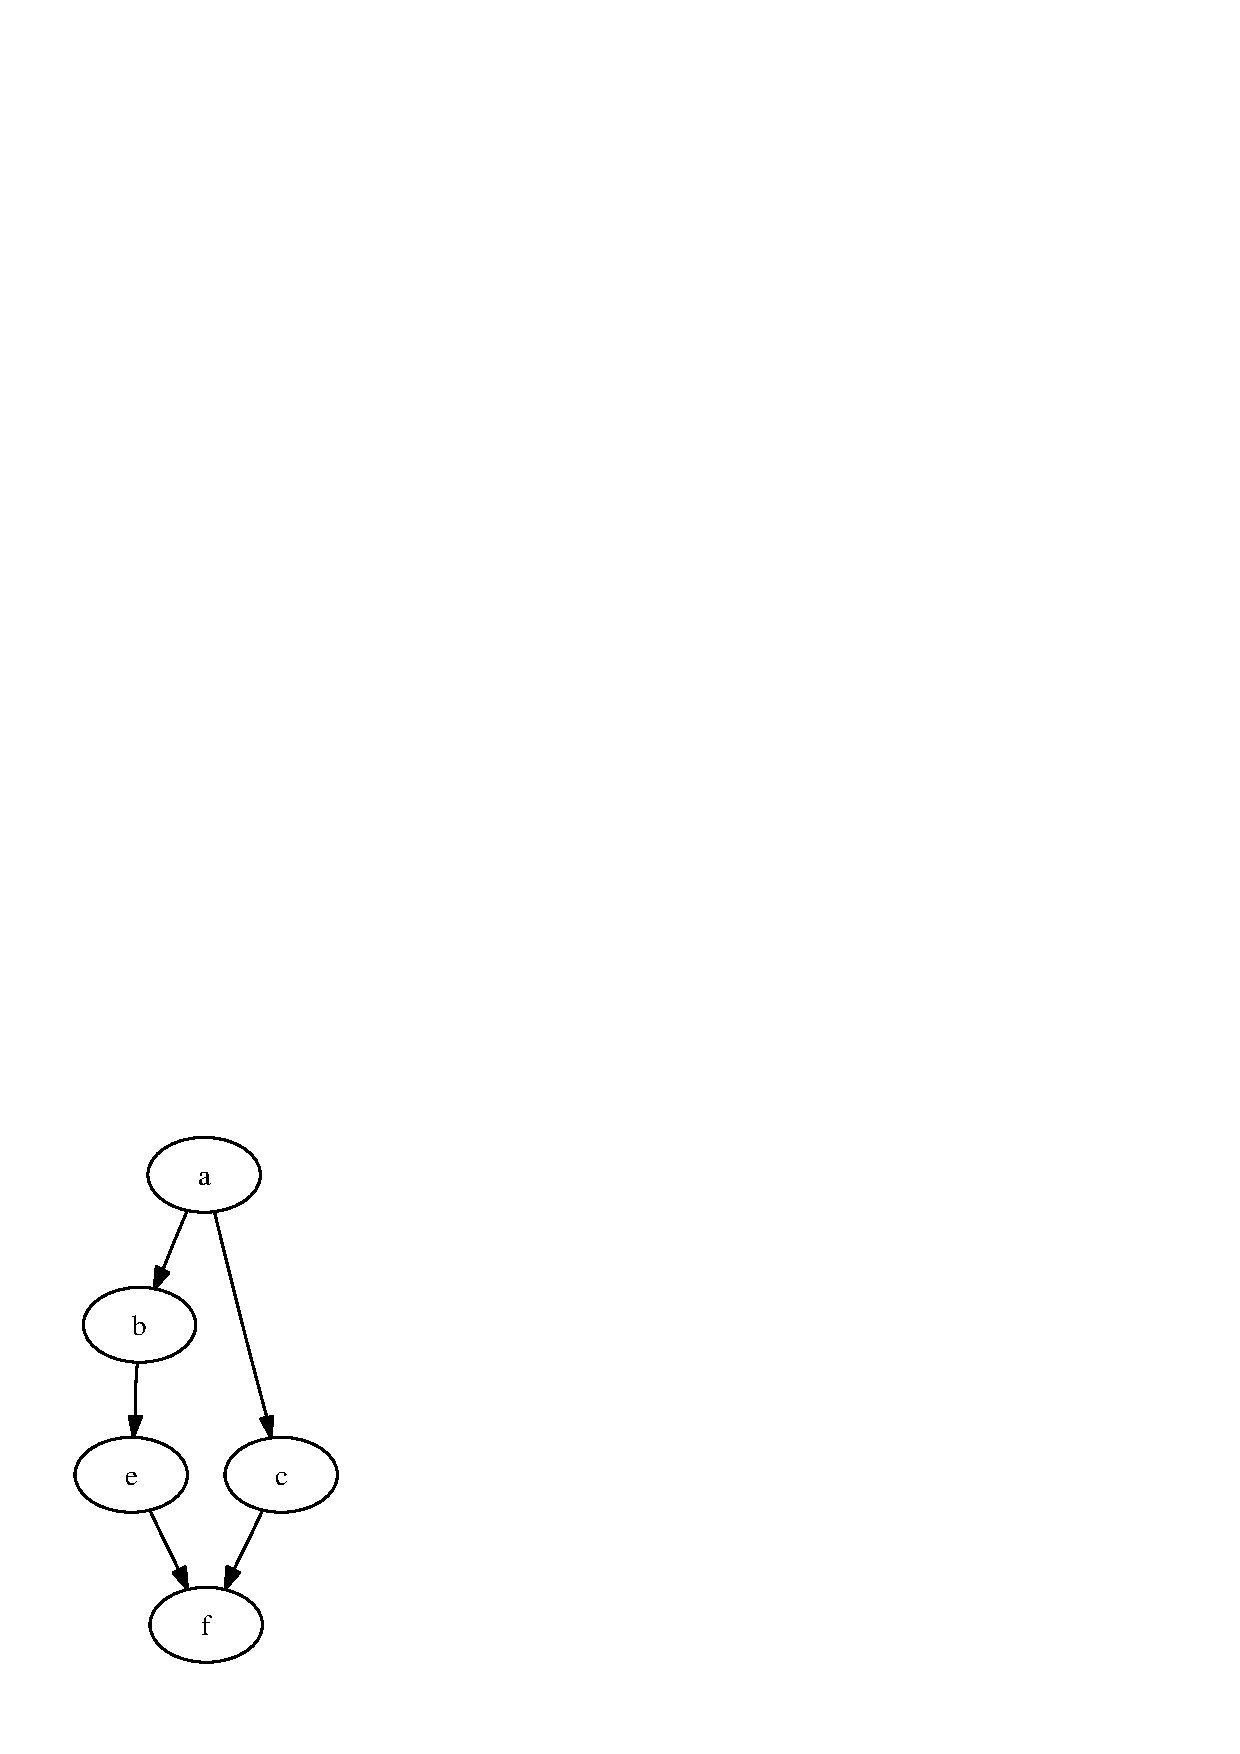
\epsfig{file=Figures/graph,scale=0.5}
  \caption{Ein einfacher Graph ohne Zykeln}
  \label{fig:graph}
\end{figure}

Wir wollen nun ein \textsl{Prolog}-Programm entwickeln, mit dem es möglich ist, für zwei
vorgegebene Knoten $x$ und $y$ zu entscheiden, ob es einen Weg von $x$ nach $y$ gibt.
Außerdem soll dieser Weg dann als Liste von Knoten berechnet werden.
Unser erster Ansatz besteht aus dem Programm, das in Abbildung \ref{fig:connect} gezeigt
ist.  Die Idee ist, dass der Aufruf \\[0.1cm]
\hspace*{1.3cm} \texttt{find\_path(\textsl{Start}, \textsl{Goal}, \textsl{Path})} \\[0.1cm]
einen Pfad \textsl{Path} berechnet, der von \textsl{Start} nach \textsl{Goal} führt.  Wir diskutieren
die Implementierung.

\begin{figure}[!h]
  \centering
\begin{Verbatim}[ frame         = lines, 
                  framesep      = 0.3cm, 
                  labelposition = bottomline,
                  numbers       = left,
                  numbersep     = -0.2cm,
                  xleftmargin   = 0.8cm,
                  xrightmargin  = 0.8cm
                ]
    % find_path( +Point, +Point, -List(Point) ).
    find_path( X, X, [ X ] ).
    
    find_path( X, Z, [ X | Path ] ) :-
        edge( X, Y ),
        find_path( Y, Z, Path ).
\end{Verbatim}
\vspace*{-0.3cm}
  \caption{Berechnung von Pfaden in einem Graphen}
  \label{fig:connect}
\end{figure}

\begin{enumerate}
\item Die erste Klausel sagt aus, dass es trivialerweise einen Pfad von \texttt{X} nach
      \texttt{X} gibt.  Dieser Pfad enthält genau den Knoten \texttt{X}.
\item Die zweite Klausel sagt aus, dass es einen Weg von \texttt{X} nach \texttt{Z}
      gibt, wenn es zunächst eine direkte Verbindung von \texttt{X} zu einem Knoten
      \texttt{Y} gibt und wenn es dann von diesem Knoten \texttt{Y} eine Verbindung
      zu dem Knoten \texttt{Z} gibt.  Wir erhalten den Pfad, der von \texttt{X} nach
      \texttt{Z} führt, dadurch, dass wir vorne an den Pfad, der von \texttt{Y} nach \texttt{Z}
      führt, den Knoten \texttt{X} anfügen.
\end{enumerate}
Stellen wir an das \textsl{Prolog}-System die Anfrage \texttt{find\_path(a,f,P)}, so
erhalten wir die Antwort
\begin{Verbatim}[ frame         = lines, 
                  framesep      = 0.3cm, 
                  labelposition = bottomline,
                  numbers       = left,
                  numbersep     = -0.2cm,
                  xleftmargin   = 0.8cm,
                  xrightmargin  = 0.8cm
                ]
    ?- find_path(a,f,P).
 
    P = [a, b, e, f] ;   
    P = [a, c, f] ;
    No
\end{Verbatim}
Durch Backtracking werden also alle möglichen Wege von \texttt{a} nach \texttt{b} gefunden.
Als nächstes testen wir das Programm mit dem in Abbildung \ref{fig:graph2} gezeigten
Graphen.  Diesen Graphen stellen wir wie folgt in \textsl{Prolog} dar:
\begin{Verbatim}[ frame         = lines, 
                  framesep      = 0.3cm, 
                  labelposition = bottomline,
                  numbers       = left,
                  numbersep     = -0.2cm,
                  xleftmargin   = 0.8cm,
                  xrightmargin  = 0.8cm
                ]
    edge(a, b).
    edge(a, c).
    edge(b, e).
    edge(e, a).
    edge(e, f).
    edge(c, f).
\end{Verbatim}

\begin{figure}[!h]
  \centering
  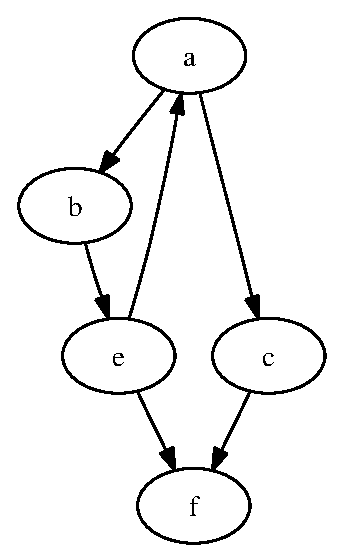
\epsfig{file=Figures/graph2,scale=0.5}
  \caption{Ein Graph mit einem Zykel}
  \label{fig:graph2}
\end{figure}

Jetzt erhalten wir auf die Anfrage \texttt{find\_path(a,f,P)} die Antwort
\begin{Verbatim}[ frame         = lines, 
                  framesep      = 0.3cm, 
                  labelposition = bottomline,
                  numbers       = left,
                  numbersep     = -0.2cm,
                  xleftmargin   = 0.8cm,
                  xrightmargin  = 0.8cm
                ]
    ?- find_path(a,f,P).
    ERROR: Out of local stack
\end{Verbatim}
Die Ursache ist schnell gefunden.
\begin{enumerate}
\item Wir starten mit der Anfrage \\[0.1cm]
      \hspace*{1.3cm} \texttt{find\_path(a,f,P)}.
\item Nach Unifikation mit der zweiten Klausel haben wir die Anfrage reduziert auf \\[0.1cm]
      \hspace*{1.3cm} 
      \texttt{edge( a, Y1 ), find\_path( Y1, f, P1 )}.
\item Nach Unifikation mit dem Fakt \texttt{edge(a,b)} haben wir die neue Anfrage \\[0.1cm]
      \hspace*{1.3cm} 
      \texttt{find\_path( b, f, P1 )}.
\item Nach Unifikation mit der zweiten Klausel haben wir die Anfrage reduziert auf \\[0.1cm]
      \hspace*{1.3cm} 
      \texttt{edge( b, Y2 ), find\_path( Y2, f, P2 )}.
\item Nach Unifikation mit dem Fakt \texttt{edge(b,e)} haben wir die neue Anfrage \\[0.1cm]
      \hspace*{1.3cm} 
      \texttt{find\_path( e, f, P2 )}.
\item Nach Unifikation mit der zweiten Klausel haben wir die Anfrage reduziert auf \\[0.1cm]
      \hspace*{1.3cm} 
      \texttt{edge( e, Y3 ), find\_path( Y3, f, P3 )}.
\item Nach Unifikation mit dem Fakt \texttt{edge(e,a)} haben wir die neue Anfrage \\[0.1cm]
      \hspace*{1.3cm} 
      \texttt{find\_path( a, f, P3 )}.
\end{enumerate}
Die Anfrage ``\texttt{find\_path(a, f, P3)}'' unterscheidet sich von der ursprünglichen
Anfrage ``\texttt{find\_path(a,f,P)}'' nur durch den Namen der Variablen.  Wenn wir jetzt
weiterrechnen würden, würde sich die Rechnung nur wiederholen, ohne dass wir vorwärts kommen.
Das Problem ist, das \textsl{Prolog} immer die erste
Klausel nimmt, die passt.  Wenn später die Reduktion der Anfrage scheitert, wird zwar nach
Backtracking die nächste Klausel ausprobiert, aber wenn das Programm in eine
Endlos-Schleife läuft, dann gibt es eben kein Backtracking, denn das Programm weiß ja
nicht, dass es in einer Endlos-Schleife ist.

Es ist leicht das Programm so umzuschreiben, dass keine Endlos-Schleife mehr
auftreten kann.  Die Idee ist, dass wir uns merken, welche Knoten wir bereits besucht
haben und diese nicht mehr auswählen.  In diesem Sinne implementieren wir nun ein Prädikat \texttt{find\_path/4}.
Die Idee ist, dass der Aufruf \\[0.1cm]
\hspace*{1.3cm} \texttt{find\_path(\textsl{Start}, \textsl{Goal}, \textsl{Visited}, \textsl{Path})} \\[0.1cm]
einen Pfad berechnet, der von \textsl{Start} nach \textsl{Goal} führt und der zusätzlich
keine Knoten benutzt, die bereits in der Liste \textsl{Visited} aufgeführt sind.  Diese Liste
füllen wir bei den rekursiven Aufrufen nach und nach mit den Knoten an, die wir bereits
besucht haben.  Mit Hilfe dieser Liste vermeiden wir es, einen Knoten zweimal zu besuchen.
Abbildung \ref{fig:connect2} zeigt die Implementierung.
\begin{figure}[!h]
  \centering
\begin{Verbatim}[ frame         = lines, 
                  framesep      = 0.3cm, 
                  labelposition = bottomline,
                  numbers       = left,
                  numbersep     = -0.2cm,
                  xleftmargin   = 0.8cm,
                  xrightmargin  = 0.8cm
                ]
    % find_path( +Point, +Point, +List(Point), -List(Point) )

    find_path( X, X, _Visited, [ X ] ).
    
    find_path( X, Z, Visited, [ X | Path ]) :-
        edge( X, Y ),
        \+ member( Y, Visited ),
        find_path( Y, Z, [ Y | Visited ], Path ).
    \end{Verbatim}
\vspace*{-0.3cm}
  \caption{Berechnung von Pfaden in zyklischen Graphen}
  \label{fig:connect2}
\end{figure}
\begin{enumerate}
\item In der ersten Klausel spielt das zusätzliche Argument noch keine Rolle,
      denn wenn wir das Ziel erreicht haben, ist es uns egal, welche Knoten wir schon
      besucht haben.
\item In der zweiten Klausel überprüfen wir in Zeile 7, ob der Knoten \texttt{Y}
      in der Liste \textsl{Visited}, die die Knoten enthält, die bereits besucht wurden,
      auftritt.  Nur wenn dies nicht der Fall ist, versuchen wir rekursiv von \texttt{Y}
      einen Pfad nach \texttt{Z} zu finden.  Bei dem rekursiven Aufruf erweitern wir die Liste
      \texttt{Visited} um den Knoten \texttt{Y}, denn diesen Knoten wollen wir in Zukunft
      ebenfalls vermeiden.
\end{enumerate}
Mit dieser Implementierung ist es jetzt möglich, auch in dem zweiten Graphen einen Weg von
\texttt{a} nach \texttt{f} zu finden, wir erhalten folgendes Ergebnis:
\pagebreak

\begin{Verbatim}[ frame         = lines, 
                  framesep      = 0.3cm, 
                  labelposition = bottomline,
                  numbers       = left,
                  numbersep     = -0.2cm,
                  xleftmargin   = 0.8cm,
                  xrightmargin  = 0.8cm
                ]
    ?- find_path(a,f,[a],P).
    P = [a, b, e, f] ;
    P = [a, c, f] ;    
    No
\end{Verbatim}


\subsection{Die Bekehrung der Ungläubigen}
Als spielerische Anwendung zeigen wir nun, wie sich mit Hilfe des oben definierten Prädikats 
\texttt{find\_path/4} ein theologisches Problem lösen lässt.
\vspace*{0.3cm}

\begin{minipage}[c]{14cm}
{\sl Drei Missionare und drei Ungläubige wollen zusammen einen Fluss 
überqueren. Sie haben nur ein Boot, indem maximal zwei Passagiere fahren können.  
Sowohl die Ungläubigen als auch die Missionare können rudern.
Weder die Gläubigen, noch die Ungläubigen können über das Wasser laufen.
Die Ungläubigen sind hungrig, wenn die Missionare an einem der Ufer in der Unterzahl sind, 
haben sie ein Problem.  Die Aufgabe besteht darin, einen Fahrplan zu 
erstellen, so dass hinterher alle das andere  Ufer erreichen und die
Missionare zwischendurch kein Problem haben.}
\end{minipage}
\vspace*{0.4cm}

\noindent
Die Idee ist, das Rätsel, durch einen Graphen zu modellieren.  Die Knoten dieses 
Graphen sind dann die Situationen, die während des Übersetzens auftreten.  Wir
repräsentieren diese Situationen durch Terme der Form \\[0.1cm]
\hspace*{1.3cm} $\texttt{side}(M,\;K,\;B)$.
\\[0.1cm]
Ein solcher Term repräsentiert eine Situation, bei der auf der linken Seite des Ufers $M$ Missionare, $K$
Ungläubige und $B$ Boote sind.  Unsere Aufgabe besteht nun darin, das Prädikat
\texttt{edge/2} so zu implementieren, dass \\[0.1cm]
\hspace*{1.3cm} $\texttt{edge}(\;\texttt{side}(M_1,\;K_1,\;B_1),\;\texttt{side}(M_2,\;K_2,\;B_2)\;)$
\\[0.1cm]
genau dann wahr ist, wenn die Situation $\texttt{side}(M_1,\;K_1,\;B_1)$
durch eine Boots-Überfahrt in die Situation $\texttt{side}(M_2,\;K_2,\;B_2)$ überführt
werden kann und wenn zusätzlich die Missionare in der neuen Situation kein Problem bekommen.
Abbildung \ref{fig:missionare.pl} auf Seite \pageref{fig:missionare.pl}
zeigt ein \textsl{Prolog}-Programm, was das Rätsel löst.  Den von diesem Programm
berechneten Fahrplan finden Sie in Abbildung \ref{fig:missionare-solution} 
auf Seite \pageref{fig:missionare-solution}.
Wir diskutieren dieses Programm nun Zeile für Zeile.

\begin{figure}[!h]
  \centering
\begin{Verbatim}[ frame         = lines, 
                  framesep      = 0.3cm, 
                  labelposition = bottomline,
                  numbers       = left,
                  numbersep     = -0.2cm,
                  xleftmargin   = 0.8cm,
                  xrightmargin  = 0.8cm
                ]
    MMM   KKK   B      |~~~~~|                   
                       >  KK >
    MMM   K            |~~~~~|      B    KK      
                       <  K  <
    MMM   KK    B      |~~~~~|            K      
                       >  KK >
    MMM                |~~~~~|      B   KKK      
                       <  K  <
    MMM   K     B      |~~~~~|           KK      
                       > MM  >
    M     K            |~~~~~|      B    KK    MM
                       < M K <
    MM    KK    B      |~~~~~|            K     M
                       > MM  >
          KK           |~~~~~|      B     K   MMM
                       <  K  <
          KKK   B      |~~~~~|                MMM
                       >  KK >
          K            |~~~~~|      B    KK   MMM
                       <  K  <
          KK    B      |~~~~~|            K   MMM
                       >  KK >
                       |~~~~~|      B   KKK   MMM
\end{Verbatim}
\vspace*{-0.3cm}
  \caption{Fahrplan für Missionare und Ungläubige}
  \label{fig:missionare-solution}
\end{figure}      

\begin{figure}[!h]
  \centering
\begin{Verbatim}[ frame         = lines, 
                  framesep      = 0.3cm, 
                  labelposition = bottomline,
                  numbers       = left,
                  numbersep     = -0.2cm,
                  xleftmargin   = 0.8cm,
                  xrightmargin  = 0.8cm
                ]
    solve :-
        find_path( side(3,3,1), side(0,0,0), [ side(3,3,1) ], Path ),
        nl, write('Lösung:' ), nl, nl,
        print_path(Path).
    
    % edge( +Point, -Point ).    
    % This clause describes rowing from the left side to the right side.
    edge( side( M, K, 1 ), side( MN, KN, 0 ) ) :-
        between( 0, M, MB ),    % MB missionaries in the boat
        between( 0, K, KB ),    % KB infidels in the boat
        MB + KB >= 1,           % boat must not be empty
        MB + KB =< 2,           % no more than two passengers
        MN is M - MB,           % missionaries left on the left side
        KN is K - KB,           % infidels left on the left side
        \+ problem( MN, KN ).   % no problem must occur
    
    % This clause describes rowing from the right side to the left side.
    edge( side( M, K, 0 ), side( MN, KN, 1 ) ) :-
        otherSide( M, K, MR, KR ),
        edge( side( MR, KR, 1 ), side( MRN, KRN, 0 ) ),
        otherSide( MRN, KRN, MN, KN ).
    
    % otherSide( +Number, +Number, -Number, -Number ).
    otherSide( M, K, M_Other, K_Other ) :-
        M_Other is 3 - M,
        K_Other is 3 - K.
    
    % problem( +Number, +Number).
    problem(M, K) :- 
            problemSide(M, K).
    
    problem(M, K) :-
        otherSide( M, K, M_Other, K_Other ),
        problemSide(M_Other, K_Other).
        
    % problemSide( +Number, +Number).
    problemSide(Missionare, Kannibalen) :- 
            Missionare > 0, 
            Missionare < Kannibalen.
    
    % find_path( +Point, +Point, +List(Point), -List(Point) )
    find_path( X, X, _Visited, [ X ] ).
    
    find_path( X, Z, Visited, [ X | Path ]) :-
            edge( X, Y ),
            \+ member( Y, Visited ),
            find_path( Y, Z, [ Y | Visited ], Path ).
\end{Verbatim}
\vspace*{-0.3cm}
  \caption{Die Bekehrung der Ungläubigen}
  \label{fig:missionare.pl}
\end{figure}      

\begin{enumerate}
\item Wir beginnen mit dem  Hilfs-Prädikat \texttt{otherSide/4}, das in den
      Zeilen 24 -- 26 implementiert ist.  Für eine vorgegebene Situation
      $\texttt{side}(M,K,B)$ berechnet der Aufruf \\[0.1cm]
      \hspace*{1.3cm} $\texttt{otherSide}(\; \texttt{side}(M, K, B),\; \textsl{OtherSide} \;)$
      \\[0.1cm] 
      einen Term, der die Situation am gegenüberliegenden Ufer beschreibt.
      Wenn an einen Ufer $M$ Missionare sind, so sind am anderen Ufer die restlichen
      Missionare und da es insgesamt $3$ Missionare gibt, sind das $3 - M$.
      Die Anzahl der Ungläubige am gegenüberliegenden Ufer wird analog berechnet. 
\item Das Prädikat \texttt{problem/2} in den Zeilen 29 -- 34 überprüft, ob es bei einer vorgegeben
      Anzahl von Missionaren und Ungläubige zu einem Problem kommt.
      Da das Problem entweder am linken oder am rechten Ufer auftreten kann,
      besteht die Implementierung aus zwei Klauseln.  Die erste Klausel prüft,
      ob es auf der Seite, an der $M$ Missionare und $K$ Ungläubige sind, zum Problem
      kommt.  Die zweite Klausel überprüft, ob es auf dem gegenüberliegenden
      Ufer zu einem Problem kommt.  Als Hilfs-Prädikat verwenden wir hier das Prädikat
      \texttt{problemSide/2}.  Dieses Prädikat ist in Zeile 37 implementiert
      und überprüft die Situation an einer Seite:  Falls sich auf einer Seite $M$ Missionare
      und $K$ Ungläubige befinden, so gibt es dann ein Problem, wenn die Zahl $M$ von 0
      verschieden ist und wenn zusätzlich $M < K$ ist.
\item Bei der Implementierung des Prädikats \texttt{edge/2} verwenden wir in den Zeilen 9
      und 10 das Prädikat \texttt{between/3}, das in dem \textsl{SWI-Prolog}-System 
      vordefiniert ist.  Beim Aufruf \\[0.1cm]
      \hspace*{1.3cm} $\texttt{between}(\textsl{Low}, \textsl{High}, N)$ \\[0.1cm]
      sind \textsl{Low} und \textsl{High} ganze Zahlen mit $\textsl{Low} \leq \textsl{High}$.
      Der Aufruf instantiert die Variable $N$ nacheinander mit den Zahlen \\[0.1cm]
      \hspace*{1.3cm} $\textsl{Low},\; \textsl{Low}+1,\; \textsl{Low}+2, \cdots, \;\textsl{High}$. \\[0.1cm]
      Beispielsweise gibt die Anfrage \\[0.1cm]
      \hspace*{1.3cm} \texttt{between(1,3,N), write(N), nl, fail.}  \\[0.1cm]
      nacheinander die Zahlen 1, 2 und 3 am Bildschirm aus.
    \item Die Implementierung des Prädikats \texttt{edge/2} besteht aus zwei Klauseln.  In
      der ersten Klausel betrachten wir den Fall, dass das Boot am linken Ufer ist.  In
      der Zeilen 9 generieren wir die Zahl der Missionare $\texttt{MB}$, die im Boot übersetzen
      sollen.  Diese Zahl $\texttt{MB}$ ist durch $\texttt{M}$ beschränkt, denn es können nur die Missionare
      übersetzen, die sich am linken Ufer befinden.  Daher benutzen wir das Prädikat
      \texttt{between/3} um eine Zahl zwischen 0 und $\texttt{M}$ zu erzeugen.  Analog generieren
      wir in Zeile 10 die Zahl $\texttt{KB}$ der Ungläubige, die im Boot übersetzen.  In Zeile 11
      testen wir, dass es mindestens einen Passagier gibt, der mit dem Boot übersetzt und
      in Zeile 12 testen wir, dass es höchstens zwei Passagiere sind.  In Zeile 13 und 14
      berechnen wir die Zahl $\texttt{MN}$ der Missionare und die Zahl $\texttt{KN}$ der Ungläubige, die
      nach der Überfahrt auf dem linken Ufer verbleiben und testen dann in Zeile 15, dass es
      für diese Zahlen kein Problem gibt.
      
      Die zweite Klausel befasst sich mit dem Fall, dass das Boot am rechten Ufer liegt.
      Wir hätten diese Klausel mit \textsl{Copy \& Paste} aus der vorhergehenden Klausel
      erzeugen können, aber es ist eleganter, diesen Fall auf den vorhergehenden Fall
      zurück zu führen.  Da da Boot nun auf der rechten Seite liegt, berechnen wir daher
      in Zeile 19 die Zahl $\texttt{MR}$ der Missionare auf der rechten Seite und die Zahl
      $\texttt{KR}$ der Ungläubige auf der rechten Seite.  Dann untersuchen wir die
      Situation $\mathtt{side}(\mathtt{MR}, \mathtt{KR}, 1)$, bei der $\texttt{MR}$
      Missionare und $\texttt{KR}$ Ungläubige am linken Ufer stehen.  Wenn diese so
      übersetzen können, dass nachher $\texttt{MRN}$ Missionare und $\texttt{KRN}$
      Ungläubige am linken Ufer stehen, dann können wir in Zeile 21 berechnen, wieviele
      Missionare und Ungläubige sich dann am gegenüberliegenden Ufer befinden.
\item In den Zeilen 1 -- 4 definieren wir nun das Prädikat \texttt{solve/0}, dessen Aufruf
      das Problem löst.  Dazu wird zunächst das Prädikat \texttt{find\_path/4} 
      mit dem Start-Knoten \texttt{side(3,3,1)} und dem Ziel-Knoten \texttt{side(0,0,0)}
      aufgerufen.   Der berechnete Pfad wird dann ausgegeben mit dem Prädikat
      \texttt{print\_path/1},
      dessen Implementierung hier aus Platzgründen nicht angegeben wird.
\end{enumerate}


%%% Local Variables: 
%%% mode: latex
%%% TeX-master: "logik"
%%% End: 
